%% abtex2-modelo-trabalho-academico.tex, v-1.7.1 laurocesar
%% Copyright 2012-2013 by abnTeX2 group at http://abntex2.googlecode.com/
%%
%% This work may be distributed and/or modified under the
%% conditions of the LaTeX Project Public License, either version 1.3
%% of this license or (at your option) any later version.
%% The latest version of this license is in
%%   http://www.latex-project.org/lppl.txt
%% and version 1.3 or later is part of all distributions of LaTeX
%% version 2005/12/01 or later.
%%
%% This work has the LPPL maintenance status `maintained'.
%%
%% The Current Maintainer of this work is the abnTeX2 team, led
%% by Lauro C\'{e}sar Araujo. Further information are available on
%% http://abntex2.googlecode.com/
%%
%% This work consists of the files abntex2-modelo-trabalho-academico.tex,
%% abntex2-modelo-include-comandos and abntex2-modelo-references.bib
%%

% ------------------------------------------------------------------------
% ------------------------------------------------------------------------
% abnTeX2: Modelo de Trabalho Academico (tese de doutorado, dissertacao de
% mestrado e trabalhos monograficos em geral) em conformidade com
% ABNT NBR 14724:2011: Informacao e documentacao - Trabalhos academicos -
% Apresentacao
% ------------------------------------------------------------------------
% ------------------------------------------------------------------------

%ARQUIVO DE PREAMBULO DA TESE - PACOTES E CONFIGURA\c{C}\~{O}ES

\documentclass[
	% -- op\c{c}\~{o}es da classe memoir --
	12pt,				% tamanho da fonte
	openright,			% cap\'{\i}tulos come\c{c}am em p\'{a}g \'{\i}mpar (insere p\'{a}gina vazia caso preciso)
	oneside,			% para impress\~{a}o em verso e anverso. Oposto a oneside
	a4paper,		% tamanho do papel.
	% -- op\c{c}\~{o}es da classe abntex2 --
	%chapter=TITLE,		% t\'{\i}tulos de cap\'{\i}tulos convertidos em letras mai\'{u}sculas
	%section=TITLE,		% t\'{\i}tulos de se\c{c}\~{o}es convertidos em letras mai\'{u}sculas
	%subsection=TITLE,	% t\'{\i}tulos de subse\c{c}\~{o}es convertidos em letras mai\'{u}sculas
	%subsubsection=TITLE,% t\'{\i}tulos de subsubse\c{c}\~{o}es convertidos em letras mai\'{u}sculas
	% -- op\c{c}\~{o}es do pacote babel --
	english,			% idioma adicional para hifeniza\c{c}\~{a}o
	%french,			% idioma adicional para hifeniza\c{c}\~{a}o
	%spanish,			% idioma adicional para hifeniza\c{c}\~{a}o
	brazil,				% o \'{u}ltimo idioma \'{e} o principal do documento
	sumario=tradicional,
	]{abntex2}

% ---
% PACOTES
% ---

% ---
% Pacotes fundamentais
% ---
\usepackage{cmap}				        % Mapear caracteres especiais no PDF
\usepackage{lmodern}			      % Usa a fonte Latin Modern			
\usepackage[T1]{fontenc}		    % Selecao de codigos de fonte.
\usepackage[utf8]{inputenc}		  % Codificacao do documento (convers\~{a}o autom\'{a}tica dos acentos)
\usepackage{lastpage}			      % Usado pela Ficha catalogr\'{a}fica
\usepackage{indentfirst}		    % Indenta o primeiro par\'{a}grafo de cada se\c{c}\~{a}o.
\usepackage{color}				      % Controle das cores
\usepackage[pdftex]{graphicx}	  % Inclus\~{a}o de gr\'{a}ficos
\usepackage{epstopdf}           % Pacote que converte as figuras em eps para pdf
\usepackage{lipsum}             % Pacote que gera texto dummy
\usepackage{blindtext}          % Pacote que gera texto dummy
% ---
		
% ---
% Pacotes adicionais, usados apenas no \^{a}mbito do Modelo Can\^{o}nico do abnteX2
% ---
%\usepackage{nomencl}

\let\printglossary\relax
\let\theglossary\relax
\let\endtheglossary\relax

\usepackage[nonumberlist]{glossaries} % nonnumberlist nao mostra as paginas nas quais os acronimos aparecem no texto
\usepackage{amsmath}
\usepackage{amssymb}
\usepackage{bbm}
\usepackage[chapter]{algorithm}
\usepackage{algorithmic}
\usepackage{multirow}
\usepackage{rotating}
\usepackage{pdfpages}
\usepackage{subfig}
\usepackage{booktabs}
\usepackage{pdflscape}
\usepackage{chngcntr}
\counterwithin{figure}{chapter}
\counterwithin{table}{chapter}

% ---
% Pacotes de cita\c{c}\~{o}es
% ---
\usepackage[brazilian,hyperpageref]{backref}	 % Paginas com as cita\c{c}\~{o}es na bibl
\usepackage[alf,abnt-etal-cite=2,abnt-etal-list=0,abnt-etal-text=emph]{abntex2cite}	% Cita\c{c}\~{o}es padr\~{a}o ABNT
% ---
% Pacote de customiza\c{c}\~{a}o - Unicamp
% ---
\usepackage{unicamp}
% ---
% CONFIGURA\c{C}\~{O}ES DE PACOTES
% ---

% ---
% Configura\c{c}\~{o}es do pacote backref
% Usado sem a op\c{c}\~{a}o hyperpageref de backref
\graphicspath{{eps/}}
\DeclareGraphicsExtensions{.eps}

%customiza\c{c}\~{a}o do negrito em ambientes matem\'{a}ticos
\newcommand{\mb}[1]{\mathbf{#1}}
\newcommand{\abs}[1]{\left|#1\right|}
\newcommand{\norm}[1]{\left\|#1\right\|}
\newcommand{\partialorder}{\cdot \geq}
\newcommand{\h}{\mathrm{h}}
\newcommand{\x}{\mathrm{x}}
\newcommand{\z}{\mathrm{z}}
\newcommand{\entropia}[1]{H{(#1)}}
%customiza\c{c}\~{a}o de teoremas
\newtheorem{mydef}{Defini\c{c}\~{a}o}[chapter]
\newtheorem{lemm}{Lema}[chapter]
\newtheorem{theorem}{Teorema}[chapter]
\floatname{algorithm}{Pseudoc\'{o}digo}
\renewcommand{\listalgorithmname}{Lista de Pseudoc\'{o}digos}
\newenvironment{proof}[1][Prova]{\begin{trivlist}
\item[\hskip \labelsep {\bfseries #1}]}{\end{trivlist}}
\newcommand{\qed}{\hfill \ensuremath{\Box}}

\renewcommand{\backrefpagesname}{Citado na(s) p\'{a}gina(s):~}
% Texto padr\~{a}o antes do n\'{u}mero das p\'{a}ginas
\renewcommand{\backref}{}
% Define os textos da cita\c{c}\~{a}o
\renewcommand*{\backrefalt}[4]{
	\ifcase #1 %
		Nenhuma cita\c{c}\~{a}o no texto.%
	\or
		Citado na p\'{a}gina #2.%
	\else
		Citado #1 vezes nas p\'{a}ginas #2.%
	\fi}%
% ---


% ---
% Configura\c{c}\~{o}es de apar\^{e}ncia do PDF final

% alterando o aspecto da cor azul
\definecolor{blue}{RGB}{41,5,195}

% informa\c{c}\~{o}es do PDF
\makeatletter
\hypersetup{
     	%pagebackref=true,
		pdftitle={\@title},
		pdfauthor={\@author},
    pdfsubject={\imprimirpreambulo},
	  pdfcreator={LaTeX with abnTeX2},
		pdfkeywords={abnt}{latex}{abntex}{abntex2}{trabalho acad\^{e}mico},
		hidelinks,					% desabilita as bordas dos links
		colorlinks=false,       	% false: boxed links; true: colored links
    linkcolor=blue,          	% color of internal links
    citecolor=blue,        		% color of links to bibliography
    filecolor=magenta,      	% color of file links
		urlcolor=blue,
%		linkbordercolor={1 1 1},	% set to white
		bookmarksdepth=4
}
\makeatother
% ---

% ---
% Altera as margens padrões
% ---
\setlrmarginsandblock{3cm}{2cm}{*}
\setulmarginsandblock{3cm}{2cm}{*}
\checkandfixthelayout
% ---

% ---
% Espa\c{c}amentos entre linhas e par\'{a}grafos
% ---
\linespread{1.3}

% O tamanho do par\'{a}grafo \'{e} dado por:
\setlength{\parindent}{2.0cm}

% Controle do espa\c{c}amento entre um par\'{a}grafo e outro:
\setlength{\parskip}{0.2cm}  % tente tamb\'{e}m \onelineskip

% ---
% Informacoes de dados para CAPA e FOLHA DE ROSTO
% ---
\titulo{Desenvolvimento de um rastreador estrelar para determinação de atitude de cubsat}
\autor{Hebert Wandick Parreira}
\local{Campinas}
\data{2022}
\orientador{Rodrigo Moreira Bacurau}
\coorientador[Co-orientador]{Prof. Dr. Co-orientador}
\instituicao{%
    UNIVERSIDADE ESTADUAL DE CAMPINAS
    \par
    Faculdade de Engenharia Mecanica	
    }
\tipotrabalho{Trabalho de conslução de curso}
%% O preambulo deve conter o tipo do trabalho, o objetivo, o nome da institui\c{c}\~{a}o e a \'{a}rea de concentra\c{c}\~{a}o
\preambulo{Trabalho apresentado \`{a} Faculdade de Engenharia Mecanica da Universidade Estadual de Campinas como parte dos requisitos exigidos para a obten\c{c}\~{a}o do t\'{\i}tulo de Engenheiro de Controle e automação.}
%\tipotrabalho{Disserta\c{c}\~{a}o (Mestrado)}
%\preambulo{Disserta\c{c}\~{a}o apresentada \`{a} Faculdade de Engenharia El\'{e}trica e de Computa\c{c}\~{a}o da Universidade Estadual de Campinas como parte dos requisitos exigidos para a obten\c{c}\~{a}o do t\'{\i}tulo de Mestre em Engenharia El\'{e}trica, na \'{A}rea de xxx.}
% --- 

% ---- compila o \'{\i}ndice  ----
\makeindex
%\makeglossaries
% ---
\usepackage[utf8]{inputenc}
\usepackage{float}
%\usepackage{graphicx}
%\usepackage[export]{adjustbox}

% Required package
\usepackage{amsmath,bm}

% ---- In\'{\i}cio do documento ----
\begin{document}

% Retira espa\c{c}o extra obsoleto entre as frases.
\frenchspacing

% ---- ELEMENTOS PR\'{E}-TEXTUAIS ----
%\pretextual

% --- Capa ---
\imprimircapa
% ---

% --- Folha de rosto (o * indica que haver\'{a} a ficha catalogr\'{a}fica) ---
\imprimirfolhaderosto
% ---

% --- Inserir a ficha catalogr\'{a}fica ---
%\includepdf{ficha_catalografica.pdf}

% --- Para a vers\~{a}o final, delete as linhas abaixo e insira a linha do \includepdf
 %\begin{fichacatalografica}
 %   \vspace*{\fill}
 %   \begin{center}
 %       \textsc{Inclua aqui o pdf com a ficha catalogr\'{a}fica fornecida pela BAE.}
 %   \end{center}
 %   \vspace*{\fill}
% --- --- ---
    %\includepdf{ficha-catalografica.pdf}
 %\end{fichacatalografica}
% ---

% ---

% --- Inserir folha de aprova\c{c}\~{a}o ---
%\includepdf{folha_de_assinaturas_oficial.pdf}

% Isto \'{e} um exemplo de Folha de aprova\c{c}\~{a}o, elemento obrigat\'{o}rio da NBR
% 14724/2011 (se\c{c}\~{a}o 4.2.1.3). Voc\^{e} pode utilizar este modelo at\'{e} a aprova\c{c}\~{a}o
% do trabalho. Ap\'{o}s isso, substitua todo o conte\'{u}do deste arquivo por uma
% imagem da p\'{a}gina assinada pela banca com o comando abaixo:

% --- Na vers\~{a}o final, exclua essas linhas e insira o \includepdf
%\newpage
%\vspace*{\fill}
%\begin{center}
%    \textsc{Inclua aqui a folha de assinaturas.}
%\end{center}
%\vspace*{\fill}
%\newpage
% --- --- ---
%\includepdf[pagecommand={\thispagestyle{plain}}]{folha-assinaturas.pdf}	
\cleardoublepage

% ---

%% --- Dedicat\'{o}ria ---
%\include{Dedicatoria}
%% ---

%% --- Agradecimentos ---
%\begin{agradecimentos}
%	Escreva seus agradecimentos.
    
    
%	\lipsum[1-3]
%\end{agradecimentos}

%% --- RESUMOS (em portugu\^{e}s e ingl\^{e}s --- 150 a 500 palavras

\begin{resumo}
    
    O bjetivo deste trabalho é realizar o desenvolvimento de um sistema de rastreamento estrelar, com baixo custo, baixo consumo de energia e com volume mássico e peso reduzido.
    Estas restrições e objetivos  se devem a aplicação desejada ao sistema, que será utilizado em cubesats.

    Para a realização deste objetivo, foi realizada uma ampla pesquisa na literatura científica acadêmica a respeito do assunto em questão, além disso foi utilizado um conjunto de técnicas e ferramentas de programação para garantir a qualidade do sistema final.
    
    Os resultados do trabalho estão divididos em duas partes, com a primeira constituindo um simulador estrelar e a segunda sendo o sistema de rastreamento estrelar em si. A primeira parte foi desenvolvida para auxiliar no desenvolvimento e averiguar a acurácia do sistema de rastreamento estrelar em ambiente simulado.
    
    \vspace{\onelineskip}

    \noindent\textbf{Palavras-chaves}: rastreador estrelar; cubesat; determinador de atitude.

    \vspace{\onelineskip}
    \vspace{\onelineskip}

    \begin{otherlanguage*}{english}
    \begin{center}{\ABNTEXchapterfont\huge Abstract}\end{center}

Same content of "Resumo".       

    \vspace{\onelineskip}

    \noindent\textbf{Keywords}: keyword 1; keyword 2; keyword 3. 

    \end{otherlanguage*}
\end{resumo}
%% ---



%% ---
%
%% --- Ep\'{\i}grafe  ---
%\begin{epigrafe}
%    \vspace*{\fill}
%	\begin{flushright}
%		\textit{``Escreva aqui a sua ep\'{\i}grafe''\\
%		(Cita\c{c}\~{a}o)}
%	\end{flushright}
%\end{epigrafe}
%% ---
%
%
%% --- inserir lista de ilustra\c{c}\~{o}es ---
\pdfbookmark[0]{\listfigurename}{lof}
\listoffigures*
\cleardoublepage
%% ---
%
%% --- inserir lista de tabelas ---
\pdfbookmark[0]{\listtablename}{lot}
\listoftables*
\cleardoublepage
%% ---
%
%% --- inserir lista de Acronimos e Abrevia\c{c}\~{o}es ---
%\renewcommand{\nomname}{Lista de Acr\^{o}nimos e Abrevia\c{c}\~{o}es}
%\pdfbookmark[0]{\nomname}{las}
%\printnomenclature
%\cleardoublepage
%% ---

%% --- inserir o sumario ---
\pdfbookmark[0]{\contentsname}{toc}
\tableofcontents*
\clearpage
%% ---

\pagenumbering{arabic}
\setcounter{page}{5}

% ---- ELEMENTOS TEXTUAIS ----
\textual


\chapter{Introdução}
\label{cap:Introducao_init}

Este documento apresenta o Trabalho de Graduação do aluno Hebert Wandick Parreira, que é realizado sob a orientação do Professor Dr. Rodrigo Moreira Bacurau, no curso de Engenharia de Controle e Automação do nível da graduação na Faculdade de Engenharia Mecânica da UNICAMP.

Um dos principais sistemas de um satélite é o sistema de determinação de atitude, o qual é parte do sistema de controle de atitude de um cubesat, que é responsável pela orientação espacial do satélite. Este sistema é de extrema importância, pois os cubesats podem possuir missões nas quais a orientação angular fixa é necessária ou uma variação angular controlada seja necessária, como para tirar fotos da superfície terrestre e fornecer acesso de rede a estação fixa em solo, como por exemplo, é o caso do Starlink.

Durante este projeto, será desenvolvido sistema de rastreamento estrelar para cubesat, com aplicabilidade  na indústria aeroespacial. O sistema será baseado em visão computacional. Pretende-se utilizar webcams convencionais e utilizar como unidade de processamento embarcados de baixo custo que executam Linux, como por exemplo a Raspberry Pi 4.

O foco desse projeto será no desenvolvimento dos algoritmos responsáveis por fazer a captura e análise das imagens, e determinar a posição  angular do cubesat. Para testar o sistema, será desenvolvido uma simulação. Ela consistirá de um monitor juntamente de um software  de simulação do céu estrelado a ser visualizado pelo dispositivo. 

Essa simulação, será desenvolvida em linguagem Python e permitirá a rotação em todo o espaço com 360 graus de liberdade em todos os eixos, por fim será realizada uma validação final com uma webcam.

\section{Motivação}
\label{sec:Introducao_motivacao}
Com o desenvolvimento da eletrônica, os circuitos e sistemas presentes em satélites conseguiram se tornar menores, mais leves, mais baratos, rápidos, e com maior eficiência  energética. Além disso, o desenvolvimento de uma padronização nas dimensões destes pequenos satélites possibilitou um decréscimo ainda maior de custo.

Em universidades e StartUps o estudo e desenvolvimento de cubesats vem crescendo rapidamente, mesmo que os pequenos satélites apresentem limitações físicas e energéticas, o custo benefício em sua aplicabilidade é grande.

Outra limitação está na capacidade do satélite de se localizar e orientar no espaço, ou seja, controlar a sua atitude, que devido às restrições já mencionadas, costumam ser extremamente limitados ou mesmo inexistentes ~\cite[]{Diaz}. Com isto, as possibilidades de aplicações destes cubesats tornam-se consideravelmente limitadas.

A primeira etapa para realizarmos o controle de atitude, é identificar de forma confiável, precisa e contínua a atitude do satélite ~\cite[]{Diaz}. No espaço existem pontos de referência que podem ser utilizados para a determinação da atitude, como o Sol, Lua e a Terra, porém estas referências não são consistentes, já que o Sol pode estar encoberto, e a análise da superfície terrestre vista do espaço varia muito, devido a nuvens e outros fenômenos meteorológicos. Além disso, a análise de imagens complexas é custosa computacionalmente, o que devido às limitações de volume e energia, tornam a aplicação extremamente complicada.

Outra opção é utilizar o campo magnético da terra, porém a interferência eletromagnética é algo relativamente comum, uma vez que os próprios circuitos elétricos do satélite podem gerar interferências.

Uma terceira opção é a utilização de uma câmera realizando a análise das estrelas, o fato do satélite estar no espaço faz com que as estrelas estejam na maioria do tempo no campo de visão do satélite ~\cite[]{Tappe}.

Realizar o controle de atitude apenas utilizando IMU (Inertial measurement unit)  é difícil, pois IMU são suscetíveis a erros de desvio de Offset, erros de Instabilidade, temperatura, são sensíveis a pancadas e vibrações ~\cite[]{Young}. Desta forma utiliza-se IMUs de alto custo, que são caros, e em sua maioria, grandes. 

Com a utilização de um dos três métodos de sensorialmente apresentados anteriormente, pode-se utilizar IMUs de menor custo para auxiliar o processo, e fazer fusão sensorial, pois a deriva dos giroscópios, causará erros de orientações consideráveis em poucos segundos se não houver algum outro sistema para identificação de atitude.

Devido a questões de custo e disponibilidade, utiliza-se componentes de prateleira (sensores e chips já prontos e vendidos em massa). Geralmente fazendo uso da tecnologia MEMS (micro electro mechanical systems), os quais são relativamente baratos, pequenos e possuem massa reduzida. 



%\section{Determinação da Atitude}
%\label{sec:sec01}
%Atitude de um satélite consiste em sua orientação no espaço, um satélite possui 6 graus de liberdade, (três de rotação e três de translação)  normalmente  modelados em 12 variáveis de estado: 6 variáveis de posição e 6 de suas respectivas derivadas, já que a estabilização e o controle de orientação são normalmente desejados no controle ~\cite[]{Souza}.

%Do Cálculo sabemos, que a derivada da posição a sua velocidade, e sabendo-se o valor da posição a todo instante pode-se calcular a derivada, portanto é possível facilmente obter a informação da velocidade. Desta forma, é necessário apenas a utilização de sensores de posição, o que é verdade, porém a precisão se eleva muito ao utilizarmos múltiplos sensores, e realizarmos uma fusão sensorial completa. 

%Este trabalho foca no desenvolvimento do rastreador estelar que é responsável pela determinação da rotação nos 3 eixos, já pensado para a incorporação em tais conjuntos de dados futuramente.




\chapter{Revisão bibliográfica}
\label{cap:Revisao_bibliografica_init}

Existem várias formas de se medir a atitude, porém, 
a forma mais amplamente utilizada em satélites de grande porte são os seguidores de estrelas (\textit{star trackers}). 
A tecnologia de tais sistemas vêm evoluindo nos últimos anos, com a rápida melhoria dos sensores CCD (\textit{charge-coupled device}), 
e tecnologias de análise de imagem. Porém,  erros são  inerentes a qualquer medida, por mais pequeno que um erro possa ser, pode levar a uma identificação errônea de uma estrela, resultado em um erro completo de posicionamento.

Star Trackers funcionam capturando imagens de estrelas e comparando a tabelas salvas em memória ~\cite[]{Diaz}. Desta forma, o satélite é capaz de identificar a sua atitude.

No entanto, os sistemas comerciais possuem preço elevado, consumo de energia elevado e massa elevada para pequenos satélites, como é mostrado na Figura ~\ref{fig:Comp_star_trackers_comerciais}.

\begin{figure}[!h]
	\centering
	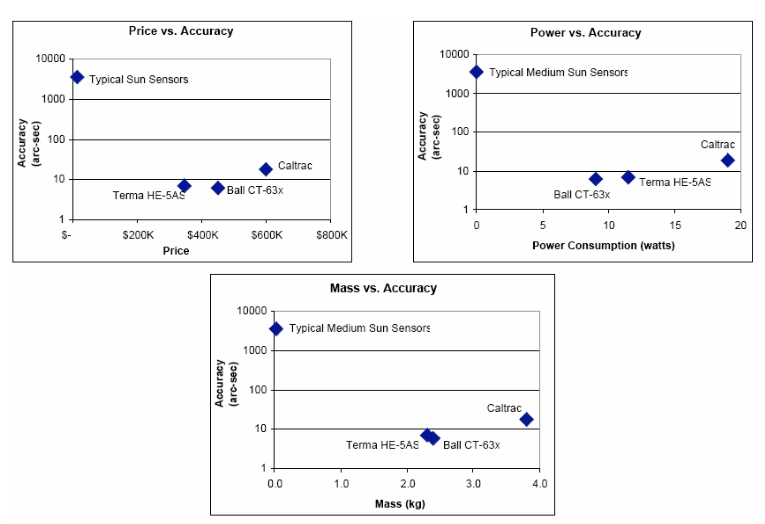
\includegraphics[width=1\columnwidth]{images/comp_star_trackers.png}
	\caption{Comparação de Star Trackers comerciais. (a) Relação entre preço e precisão, (b) Relação entre energia consumida e precisão, (c) Relação entre massa e precisão. Fonte: ~\cite[]{Diaz}}
	\label{fig:Comp_star_trackers_comerciais}
\end{figure}


\section{Etapas de operação}


As etapas de operação dos Star Tracks, em geral, seguem a estrutura apresentada na Figura ~\ref{fig:etapas_star_trackers}.


\begin{figure}[H]
	\centering
	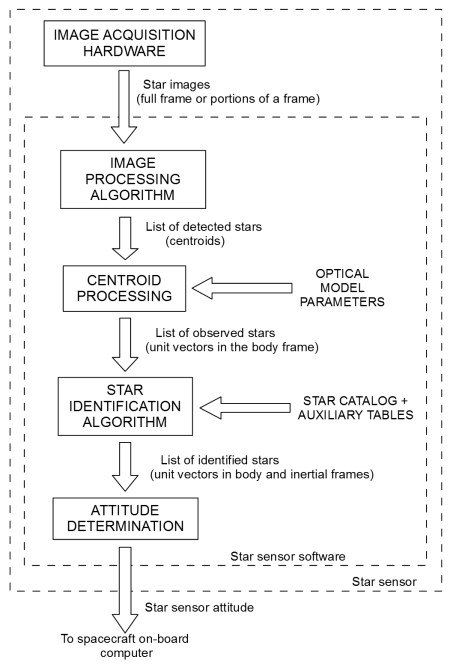
\includegraphics[width=.6\columnwidth]{images/etapas.jpg}
	\caption{Etapas de funcionamento de um Star Tracker. Fonte: ~\cite[]{Fialho}}
	\label{fig:etapas_star_trackers}
\end{figure}

A primeira etapa de operação, consiste  na aquisição da imagem a ser utilizada, para tal é utilizado um CCD acoplado a um conjunto de lentes. A escolha desse componentes deve levar em conta uma série de parâmetros, tais como: abertura do campo visual, precisão, volume, peso e outros a variar com a  missão do cubesat ~\cite[]{Carvalho}. Neste projeto a aquisição de imagens será feita com uma \textit{webcam}.

O algoritmo de processamento juntamente com processamento de centroide, são responsáveis por localizar cada uma das estrelas e determinar sua localização e intensidade.

O algoritmo de identificação de estrelas é responsável por fazer a relação entre as estrelas identificadas na observação e as estrelas contidas no banco de dados. A identificação de uma estrela envolve a análise das relações entre as diversas estrelas observadas, para tal utiliza-se algoritmos como de  \textit{Planar Triangles} ~\cite[]{Cole}.

Por fim, é determinada a atitude do cubesat, que pode ser feita utilizando ângulos de Euler ou quaternions.

Para avaliar os algoritmos desenvolvidos, foi implementado um simulador estrelar, seguindo o método demonstrado por Tappe ~\cite[]{Tappe}. 
Por fim, foram realizados testes com imagens reais obtidas por \textit{webcams}  ou câmeras de celulares.



\section{Esfera celeste}

Para aplicação no rastreador estelar, as estrelas são representadas através de uma esfera celeste, na  qual as estrelas são distribuídas em uma esfera ao redor do centro, que na aplicação de satélites é a própria Terra. 
Devido a diferença de escalas da distância das estrelas da Terra, e o tamanho da Terra, 
pode-se considerar que qualquer ponto na Terra e na órbita terrestre, estão exatamente no centro da esfera. 
O erro gerado por tal simplificação só se tornaria visível em missões em que o veículo espacial se retirasse do sistema solar, o que não é caso para Cubesats atuais \cite{Fialho}.

Também é completamente desprezado qualquer movimento que os astros tenham em relação uns aos outros, 
pois estes movimentos são praticamente nulos em nossas análises.
Isto se deve o fato de que, o quanto maior for a distância do observador a um objeto, 
menor será a variação angular para um mesmo movimento linear do objeto, 
como por exemplo pode-se observar que aviões aparentam estar extremamente lento para um observador na Terra, 
No caso do sistema estrelar, esse efeito é ainda maior, permitindo desprezar esse movimento relativo entre as estrelas sem nenhum prejuízo prático a precisão ~\cite[]{Carvalho}.

Nesta abordagem, algumas das características da Terra são representadas na esfera, como o eixo de rotação em torno de si (rotação) e os pólos geográficos, 
que são nomeados respectivamente eixo e pólos celestes. Com isto, facilita-se a localização dos astro na esfera. 
Para isto cria-se circunferências envolvendo a esfera, concorrendo nos polos (meridianos), 
com circunferências perpendiculares ao eixo de rotação (paralelos) ~\cite[]{Carvalho}.

\begin{figure}[H]
	\centering
	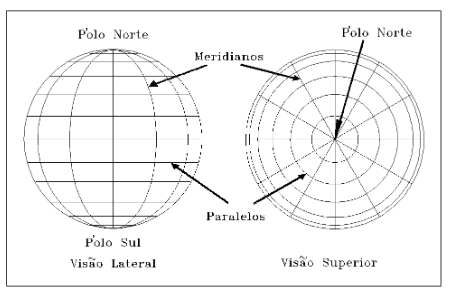
\includegraphics[width=.7\columnwidth]{images/codficacao_cod_esferas_celetes.png}
	\caption{Codificação de coordenadas na esfera celeste. Fonte: ~\cite[]{Carvalho}}
	\label{fig:codficacao_cod_esferas_celetes}
\end{figure}

Como referência tem-se o paralelo central, conhecido como paralelo do Equador,  o meridiano de referência é o que contém o ponto vernal . O ponto vernal é o momento em que o Sol passa o Equador de Sul para Norte, isto ocorre pois a rotação da Terra em torno do próprio eixo está inclinada em relação ao plano da trajetória elíptica da Terra em torno do Sol.Como é visto na Figura  ~\ref{fig:inclinacao}.

\begin{figure}[H]
	\centering
	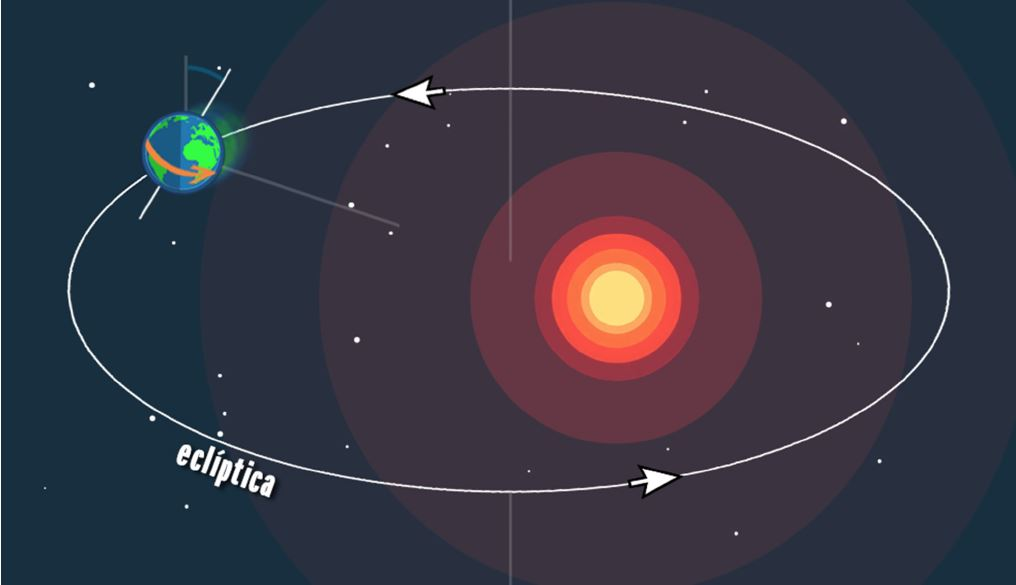
\includegraphics[width=.7\columnwidth]{images/inclinacao.jpg}
	\caption{Inclinação órbita terrestre. Fonte: ~\cite[]{Portal_do_Astronomo}}
	\label{fig:inclinacao}
\end{figure}



\section{Referencial Inercial Terrestre}

Utilizando os conceito da  Esfera Celeste, cria-se o referencial inercial terrestres, 
em que o eixo x está alinhado com vetor radial partindo do Sol em direção a Terra (linha de Áries), 
que é o equinócio de inverno, o eixo z é alinhado com o eixo de rotação da Terra, 
e o eixo y segue a regra da mão direita, conforme as figuras ~\ref{fig:Frame_inercial_terrestre} e ~\ref{fig:Referencial_inercial}.

\begin{figure}[H]
	\centering
	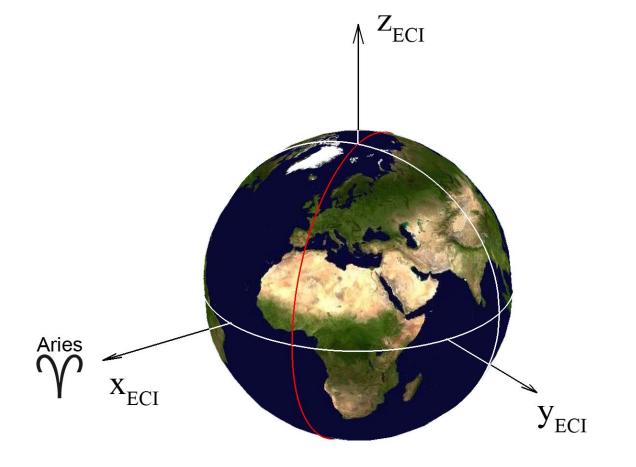
\includegraphics[width=.7\columnwidth]{images/Frame_inercial_terrestre.png}
	\caption{Frame inercial terrestre. Fonte: ~\cite[]{Diaz}}
	\label{fig:Frame_inercial_terrestre}
\end{figure}

\begin{figure}[H]
	\centering
	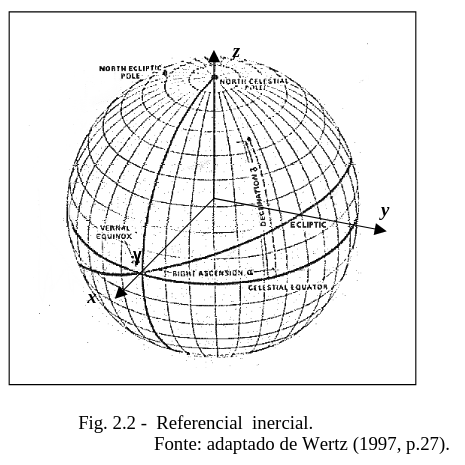
\includegraphics[width=.7\columnwidth, trim=0 60 0 0, clip=true, ]{images/Referencial_inercial.png}
	\caption{Referencial inercial. Fonte: ~\cite[]{Carvalho}}
	\label{fig:Referencial_inercial}
\end{figure}

As estrelas são catalogadas utilizando os pontos de referência, 
utilizando-se de um sistema de coordenadas polares, com duas coordenadas angulares. 
Um dos ângulos é definido a partir dos meridianos, que é a ascensão reta , o ponto de ares é o marco zero, 
a ascensão da reta, que varia de 0 a 360 graus.

A outra coordenada polar é a declinação $\gamma$, que é o ângulo entre a estrela e o paralelo do equador, 
variando de -90 a 90 graus. A Figura ~\ref{fig:Sistema_de_coordenadas_vetorial} mostra sua representação.

\begin{figure}[H]
	\centering
	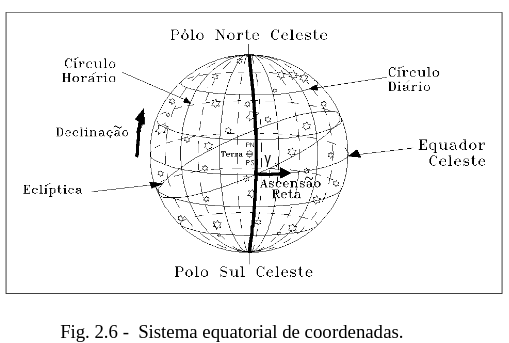
\includegraphics[width=.7\columnwidth, trim={0 30 0 0}, clip]{images/Sistema_equatorial_de_coordenadas.png}
	\caption{Sistema equatorial de coordenadas. Fonte: ~\cite[]{Carvalho}}
	\label{fig:Sistema_equatorial_de_coordenadas}
\end{figure}

A transformação do sistema de coordenadas polares para coordenadas cartesianas é feita  com base na Figura \ref{fig:Sistema_de_coordenadas_vetorial}.

\begin{figure}[H]
	\centering
	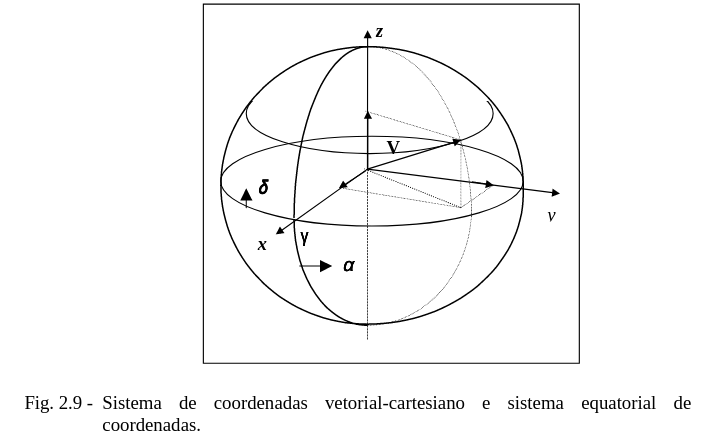
\includegraphics[width=1\columnwidth, trim={0 60 0 0}, clip]{images/Sistema_de_coordenadas_vetorial.png}
	\caption{Sistema de coordenadas vetorial- cartesiano e sistema equatorial de coordenadas. Fonte: ~\cite[]{Carvalho}}
	\label{fig:Sistema_de_coordenadas_vetorial}
\end{figure}

Todas as estrelas catalogadas são descritas na superfície de uma esfera unitária  com centro cociente a Terra, 
portanto, o módulo do vetor que sai do centro da esfera até a estrela é sempre 1,
\begin{equation}
	\left| \overrightarrow{V}\right|=1.
	\label{eq:1}
\end{equation}

Dessa forma, desconsidera-se o valor do raio nas equações de transformação de coordenadas; 
a elaboração das equações é realizada através da análise das relações trigonométricas do sistemas, 
o que resulta em:
\begin{equation}
	V_{x}=cos(\gamma)cos(\alpha),
	\label{eq:2}
\end{equation}

\begin{equation}
	V_{y}=cos(\gamma)sin(\alpha),
	\label{eq:3}
\end{equation}

\begin{equation}
	V_{z}=sin(\gamma).
	\label{eq:4}
\end{equation}


\section{Referencial do cubesat}

O referencial do cubesat é alinhado geometricamente com o equipamento, dessa forma, ele representa a posição do cubesat em si, 
como pode ser visto na Figura ~\ref{fig:Referencia_do_Cubesat}.

\begin{figure}[H]
	\centering
	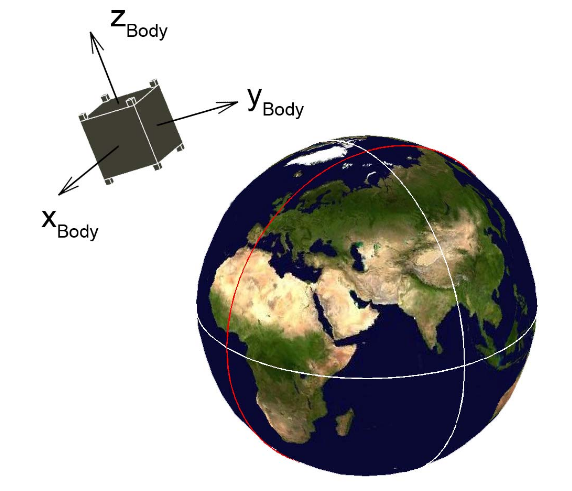
\includegraphics[width=.7\columnwidth]{images/Referencia_do_Cubesat.png}
	\caption{Referência do Cubesat. Fonte: ~\cite[]{Diaz}}
	\label{fig:Referencia_do_Cubesat}
\end{figure}

O referencial da câmera tem os eixos x e y normal ao plano da imagem, a imagem captada pela câmera se encontra a uma distância unitária do cubesat no eixo Z, o motivo de se utilizar uma distância unitária e demais informações sobre o frame de câmera, 
serão tratados no capítulo de projeções em perspectiva. Neste trabalho é considerado que o referencial do cubesat é o mesmo da câmera, como é visto na Figura ~\ref{fig:Camera_Frame}.

\begin{figure}[H]
	\centering
	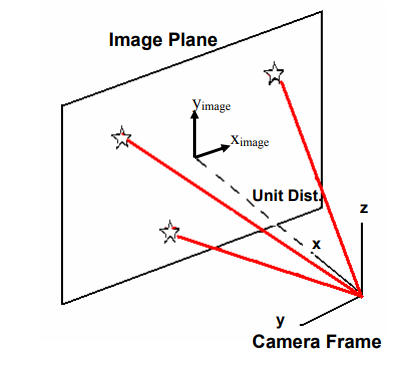
\includegraphics[width=.7\columnwidth]{images/Camera_Frame.png}
	\caption{Camera Frame. Fonte: ~\cite[]{Diaz}}
	\label{fig:Camera_Frame}
\end{figure}

\section{Catalogo de estrelas}
\label{sec:catalogo_de_estrelas}

A criação do catálogo é realizada por satélites especialmente criados e lançados com este propósito, como o é o caso do NASA I/239, que compõem o banco de dados do Hipparcos and Tycho. Este banco de dados é encontrado em ~\cite[]{ESA}.

O banco de dados possui uma tabela principal de informações, com o formato mostrado na Figura ~\ref{fig:Resumo_impetracao_parte_esquerda_Hipparcos}.

\begin{figure}[H]
	\centering
	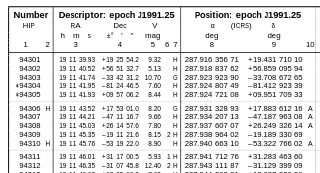
\includegraphics[width=.7\columnwidth]{images/Resumo_impetracao_parte_esquerda_Hipparcos.png}
	\caption{Resumo de impetração da parte esquerda do catálogo Hipparcos. Fonte: ~\cite[]{ESA}}
	\label{fig:Resumo_impetracao_parte_esquerda_Hipparcos}
\end{figure}

Essa tabela possui muitas informações que não serão utilizadas, incluindo uma quantidade de estrela muito grande, 
portanto o banco de dados foi filtrado com apenas alguns campos de dados restantes: número de catalogação, ascensão reta (em °), 
declinação (em °) e magnitude, que mostrado na Figura ~\ref{fig:Caracteristicas_matriz}. 
Além disto foi realizado uma filtragem por estrelas com magnitude cinco ou inferior, 
o que significa que apenas as estrelas mais brilhantes permaneceram na base de dados do sistema. 
Para a visualização das estrelas restantes utiliza-se o sistema equatorial de coordenadas, resultando nos plots apresentados nas figuras ~\ref{fig:Rrepresentacao_2D} e \ref{fig:Representacao_3D}.

\begin{figure}[H]
	\centering
	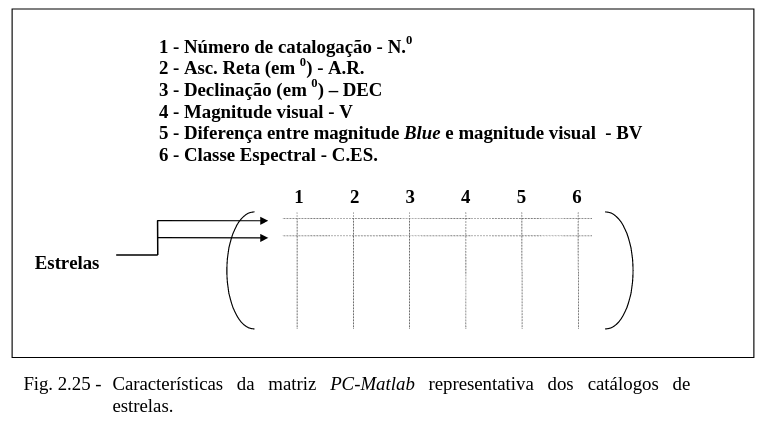
\includegraphics[width=.7\columnwidth, trim={0 60 0 0}, clip]{images/Caracteristicas_matriz.png}
	\caption{Características de matriz representativa do catálogo estelar. Fonte: ~\cite[]{Carvalho}}
	\label{fig:Caracteristicas_matriz}
\end{figure}

\begin{figure}[H]
	\centering
	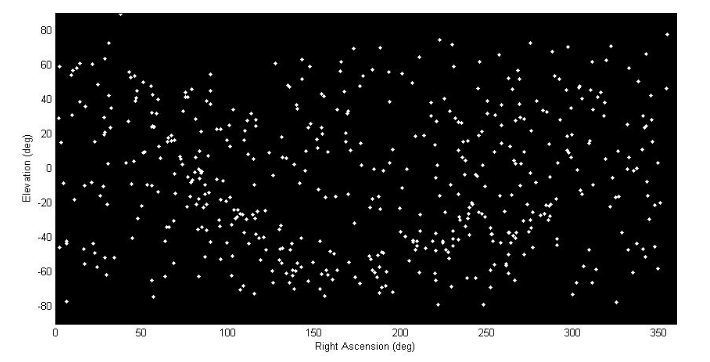
\includegraphics[width=.7\columnwidth]{images/Rrepresentacao_2D.png}
	\caption{Catálogo estelar representação em 2D. Fonte: ~\cite[]{Diaz}}
	\label{fig:Rrepresentacao_2D}
\end{figure}

\begin{figure}[H]
	\centering
	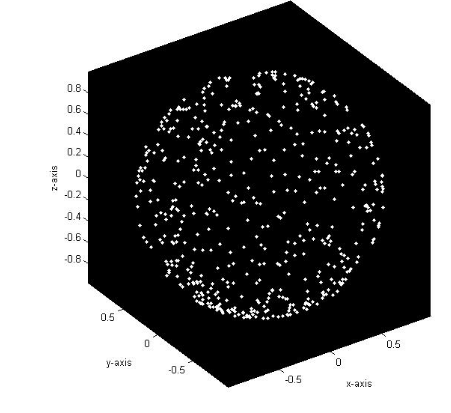
\includegraphics[width=.7\columnwidth]{images/Representacao_3D.png}
	\caption{Catálogo estelar representação em 3D. Fonte: ~\cite[]{Diaz}}
	\label{fig:Representacao_3D}
\end{figure}



\section{Análise de imagem}

Analise de imagem é o primeiro passo na analise de dados de nosso sistema, 
no caso desse trabalho a analise deve ter a capacidade de localizar a posição correta das estrelas presentes no campo de visão da câmera.
Erros nesta atapa da analise pode fazer o reconhecimento da posição angular do satélite se tornar impossível.

\subsection{Distorções em imagens}

As correções de distorções nas imagens captadas devem ser realizadas, 
com os erros não podendo ser ignorados, pois a distorção de imagem pode causar erros na localização das estrelas. 
Estas distorções se dividem em dois componentes, uma sendo a radial e outra tangencial, com a componente radial sendo predominante.
Além disto, existem distorções de construção das lentes, distorções de desalinhamento da lente em relação ao centro da Matriz CCD da câmera.

\subsubsection{Distorção radial}
Distorção radial é vista quando utiza-se câmera com grandes ângulos e com pequena distância focal~\cite[]{Mallon}.
Os efeitos da distorção radial são representados na Figura ~\ref{fig:Distorcao_radial}.

\begin{figure}[H]
	\centering
	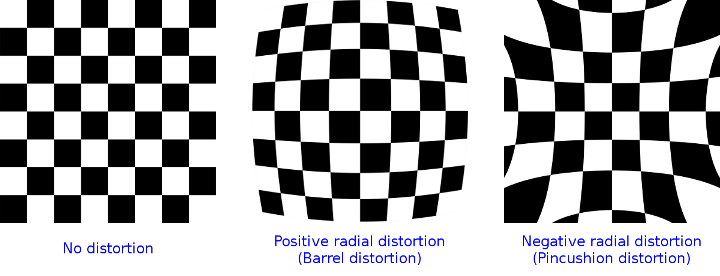
\includegraphics[width=.7\columnwidth]{images/Distorcao_radial.png}
	\caption{Distorção radial. Fonte: ~\cite[]{ozcakir_2020}}
	\label{fig:Distorcao_radial}
\end{figure}

Esta distorção pode ser corrigida através de diferentes métodos, neste trabalho utiliza-se o método matemático descrito pelo ~\cite[]{opencv_library}.
Dessa forma a distorção radial é corrigida através das equações ~\ref{eq:Distorcao_radial_x} e ~\ref{eq:Distorcao_radial_y}.

\begin{equation}
	X_{corrigido} = X_{original} (1 + k_1 r^2 + k_2 r^4 + k_3 r^6),
	\label{eq:Distorcao_radial_x}
\end{equation}

\begin{equation}
	Y_{corrigido} = Y_{original} (1 + k_1 r^2 + k_2 r^4 + k_3 r^6).
	\label{eq:Distorcao_radial_y}
\end{equation}

\subsubsection{Distorção tangencial}
Distorções tangenciais ocorrem quando a câmera e o plano da imagem não estão em paralelo ~\cite[]{ozcakir_2020}.
Os efeitos da distorção tangencial são representados na Figura ~\ref{fig:Distorcao_tangencial}.

\begin{figure}[H]
	\centering
	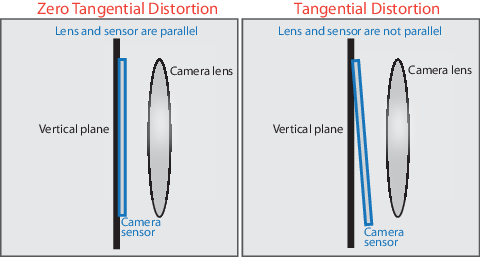
\includegraphics[width=.7\columnwidth]{images/Distorcao_tangencial.png}
	\caption{Distorção tangencial. Fonte: ~\cite[]{ozcakir_2020}}
	\label{fig:Distorcao_tangencial}
\end{figure}

Esta distorção é corrigida através das equações ~\ref{eq:Distorcao_tangencial_x} e ~\ref{eq:Distorcao_tangencial_y}.

\begin{equation}
	X_{corrigido} = X_{original} (1 + p_1 r^2 + p_2 r^4 + p_3 r^6),
	\label{eq:Distorcao_tangencial_x}
\end{equation}

\begin{equation}
	Y_{corrigido} = Y_{original} (1 + p_1 r^2 + p_2 r^4 + p_3 r^6).
	\label{eq:Distorcao_tangencial_y}
\end{equation}

Resalta-se que a ferramenta de simulação estrelar desenvolvida para este trabalho não possui distorcão tangencial, pois a câmera e o plano da imagem estão paralelos.


\section{Detecção de estrelas}
\subsection{Localização de círculos}

Os métodos de detecção de círcurlos em geral consiste nas variações do método de Hough Transform (HT), como o standard Hough Transform, 
o Fast Hough Transform de de Li et al.

Para aplicar um método de Hough Transform, é necessário se aplicar um filtro para detecção de bordas na imagem, 
que filtra apenas os pixels que estão entre na borda das estrelas detectadas, 
pois HT utiliza a posição destes pixels para calcular o possível centro do círculo.
Neste trabalho utiliza-se um filtro clássico de Canny, para realizar a detecção das bordas, 
pois o ganho em qualidade de detecção de outros algoritmos de detecção de borda, como o método de onda contínua, 
que utilizam recursos computacionais maiores, e não aumenta de forma satisfatória a qualidade de detecção de bordas, 
como é mostrado por Kobylin ~\cite[]{kobylin2014comparison}

HT faz utilização da equação do círculo, para fazer a detecção do círculo, o método consiste em se testar todas as possilidades de círculos possíveis para cada pixel na borda de cada ponto na imagem.
Uma vez feito todos os câlculos para cada um dos pixels de borda, o mêtodo seleciona o circulo com maior recorrência em diferentes pixels. Yuen demonstra sua aplicação em diferentes variações ~\cite[]{YUEN199071}.

\subsection{Transformação de coordenadas}

A localização das estrelas ocorre em coordenadas cartesianas em relação ao centro do campo de visão da câmera, 
utilizando o referêncial já demonstrado, porém é mais conveniente que a localização seja representada através de coordenadas polares, 
para isso é necessário se realizar a transformação de coordenadas.
Seguindo as formulas  ~\ref{eq:transformacao_cordenadas_theta} e ~\ref{eq:transformacao_cordenadas_r}.

\begin{equation}
	\theta  = 
	\begin{cases}
		\arctan \left( \frac{y}{x} \right), & \text{se } x >= 0 \\
		\arctan \left( \frac{y}{x} \right) + \pi, & \text{se } x < 0, \\
	\end{cases}
	\label{eq:transformacao_cordenadas_theta}
\end{equation}

\begin{equation}
	r = \sqrt{x^2 + y^2}.
	\label{eq:transformacao_cordenadas_r}
\end{equation}

A variável \textbf{r} é então transformada em uma variável ângular, através de uma relação linear. 
Com os coeficientes sendo calculados através de uma imagem de referência, 
basicamente se faz uma contagem de quantos pixels que se precisa para se percorrer 1 grau de ângulo, para se realizar a medição deste coeficiente,
na Equação ~\ref{eq:transformacao_cordenadas_theta_angular}, r é quantidade de pixels medida na imagem, e C é o coeficiente de transformação, 
\begin{equation}
	r_{angular} = r * C_{converção}.
	\label{eq:transformacao_cordenadas_theta_angular}
\end{equation}

\subsection{Cálculo do ângulos entre estrelas}

O calculo da distância entre as estrelas presentes no FOV é realizado através da Equação ~\ref{eq:calculo_distancia_estrelas}.
Além disto, é aplicado um valor máximo para limitar o ângulo entre as estrelas, pois isto diminui a quantidade de relações armazenadas no banco de dados.
Na Figura ~\ref{fig:angulo_entre_estrelas} é demonstrado as relações entre as estrelas.

\begin{figure}[H]
	\centering
	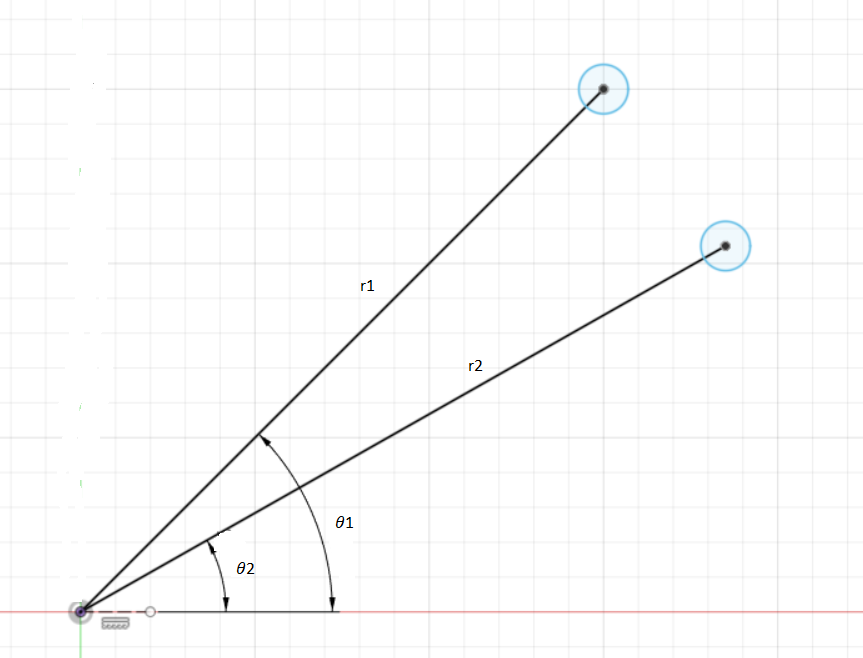
\includegraphics[width=0.5\textwidth]{images/relacoes_entre_estrelas.png}
	\caption{Relação entre estrelas no FOV da câmera, Fonte: Autoria própria}
	\label{fig:angulo_entre_estrelas}
\end{figure}

\begin{equation}
	dist_{angular} = \sqrt{r_{estrela_1}^2 + r_{estrela_2}^2 - 2 * r_{estrela_1} * r_{estrela_2} * cos(\theta_{estrela_1} - \theta_{estrela_2})}
	\label{eq:calculo_distancia_estrelas}
\end{equation}

\subsection{Cálculo da área antre estrelas}

Além da relação angular entre duas estrelas, pode-se calcular a área entre 3 estrelas, 
isto sé faz necessario pois existe uma quantidade grande de estrelas que possuem uma mesma quantidade de estrelas vizinhas a uma mesma distância angular.
Portanto utilizamos uma terceira estrela para se calcular a área entre as estrelas, que é utilizada para refinar as possíveis estrelas no campo de visão.
Para esta calculo é utilizado a fórmula de Heron ~\ref{eq:calculo_area_estrelas}, que pode ser calculada através da distância angular entre as estrelas.
Que já foi calculada na Equação ~\ref{eq:calculo_distancia_estrelas}, previamente executada pelo algoritmo.

\begin{equation}
	area = \sqrt{p(p-a)(p-b)(p-c)},
	\label{eq:calculo_area_estrelas}
\end{equation},
em que \textbf{p} é a metade do perímetro do triângulo, e \textbf{a}, \textbf{b} e \textbf{c} são as distâncias entre as estrelas.

\begin{equation}
	p = \frac{a+b+c}{2}
	\label{eq:calculo_area_estrelas_p}
\end{equation}

Esta divisão do passos para se calcular a área entre as estrelas, 
é realizada pois o calculo do momento entre a estrelas também utiliza o valor \textbf{p}.

\subsection{Cálculo do momento entre estrelas}

Uma filtragem de terceiro grau é realizada para se diminuir ainda mais a quantidade de possíveis estrelas, 
para isso utiliza-se o momento entre as estrelas, que é calculado através da Equação ~\ref{eq:calculo_momento_estrelas},

\begin{equation}
	momento = \frac{area (a^2 + b^2 + c^2)}{36}.
	\label{eq:calculo_momento_estrelas}
\end{equation}

Pode-se utilizar o momento como uma elemento extra de filtragem pois triângulos com areas semelhantes, podem possuir momentos completamente diferentes, como demonstrado na Figura ~\ref{fig:comparacao_entre_triangulos}.

\begin{figure}[H]
	\centering
	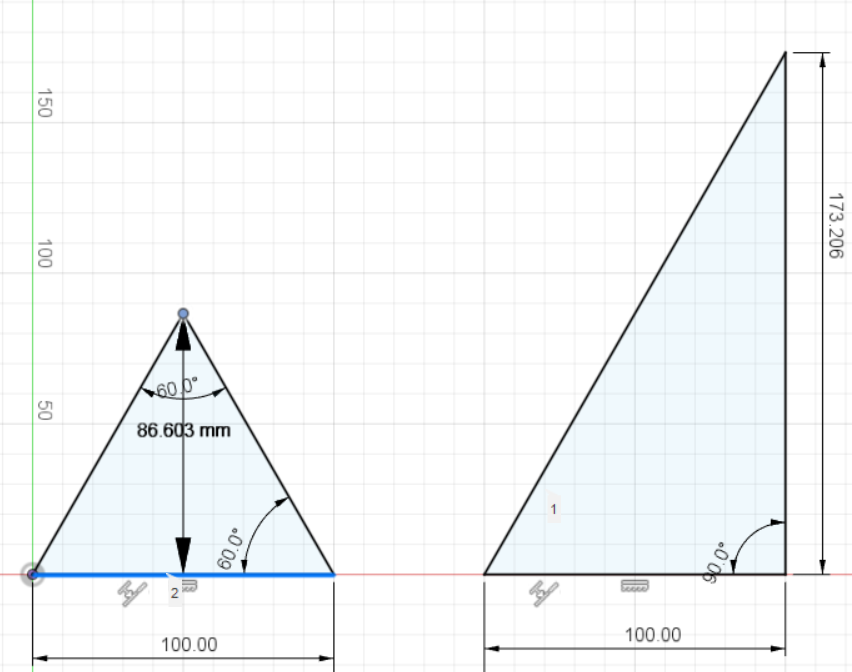
\includegraphics[width=0.5\textwidth]{images/comparacao_entre_triangulos.png}
	\caption{Relação entre estrelas no FOV da câmera, Fonte: Autoria própria}
	\label{fig:comparacao_entre_triangulos}
\end{figure}
Nota-se que esta filtragem é de custo computacional baixo, e utiliza apenas estrelas já analisadas anteriormente, 
portanto é uma passo extra eficaz e de baixo custo computacional.


\section{Banco de dados}

Feita a analise das relações geométricas entre as estrelas presentes no FOV, com as informações, de momentos, áreas e momentos angulares, 
é então inicializado a pesquisa no banco de dados interno do cubesat, para verificarão de possíveis estrelas.

Devido às limitações energéticas do sistema, é necessário que a estrutura do banco de dados seja otimizada para a resolução do problema em questão.
Além disto o próprio processo de geração do banco de dados que também requer uma otimização, para que o mesmo seja gerado em um tempo aceitável.
Pois, a combinação de 3 estrelas diferentes para realização do calculo da area e do momento pode gerar um problema de O(n\textsuperscript{3}).

Além disto a técnicas de busca e analise de resultados também devem ser otimizadas e levar levar em consideração múltiplos fatores.
Cabe ressaltar que a operação do sistema de orientação e controle do cubesat possui duas fases distintas de operação, a fase em que não há informação previa de localização e a fase em que já há informação previa de localização.
Neste trabalho é apenas abordada a fase em que não há informação previa de localização.

\subsection{Gerando o banco de dados}
Após a análise de imagem o sistema precisa compar os resultados das leituras com um banco de dados de estrelas, para que seja possível identificar a posição do cubesat, 
relacionando a posição da estrela observada a posição do cubesat, 
o banco de dados é composto por algumas partes, sendo elas:
\begin{itemize}
    \item \textbf{Relações Áreas e Momentos angulares}: Lista ordenada da combinação de 3 estrelas. Contendo as informações de área e momento angular, juntamente com o identificador das estrelas Figura \ref{fig:banco_dados_area_moment_to_cubesat}.
    \item \textbf{Relações de Ângulos entre estrelas}: Lista ordenada da combinação de 2 estrelas. Contendo as informações de ângulo entre as estrelas, juntamente com o identificador das estrelas Figura \ref{fig:banco_dados_angulo}.
    \item \textbf{Relação de id e posição estrelar}: Este é o mesmo banco de dados utilizado para gerar a simulação, contendo as informações de id e posição estrelar Figura \ref{fig:banco_dados_posicao}.
\end{itemize}

\begin{figure}[H]
    \centering
    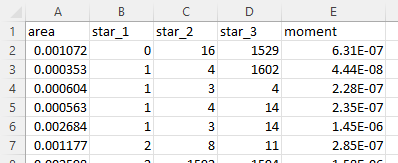
\includegraphics[width=0.7\textwidth]{images/banco_dados_area_moment.png}
    \caption{Parte do arquivo de banco de dados de áreas e momentos angulares, Fonte: Autoria própria}
    \label{fig:banco_dados_area_moment_to_cubesat}
\end{figure}

\begin{figure}[H]
    \centering
    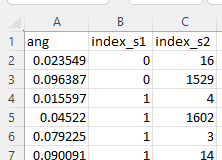
\includegraphics[width=0.35\textwidth]{images/banco_dados_angulo.png}
    \caption{Parte do arquivo de banco de dados de ângulos entre estrelas, Fonte: Autoria própria}
    \label{fig:banco_dados_angulo}
\end{figure}

\begin{figure}[H]
    \centering
    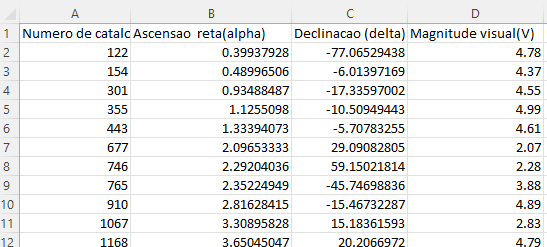
\includegraphics[width=0.7\textwidth]{images/banco_dados_posicao.png}
    \caption{Parte do arquivo de banco de dados de posição estrelar, Fonte: Autoria própria}
    \label{fig:banco_dados_posicao}
\end{figure}

\subsubsection{Octree}

Nota-se que a combinação de 3 estrelas diferentes para realização do cálculo da área e do momento pode gerar um problema de complexabilidade O(n\textsuperscript{3}),
Porém, apenas estrelas próximas uma as outras que podem geram uma combinação de area valida para a analise.
Nota-se que apenas estrelas dentro de um circulo ao redor da estrela central podem gerar uma combinação de area valida para a analise, como visto na Figura \ref{fig:estrelas_endorno}.

\begin{figure}[H]
    \centering
    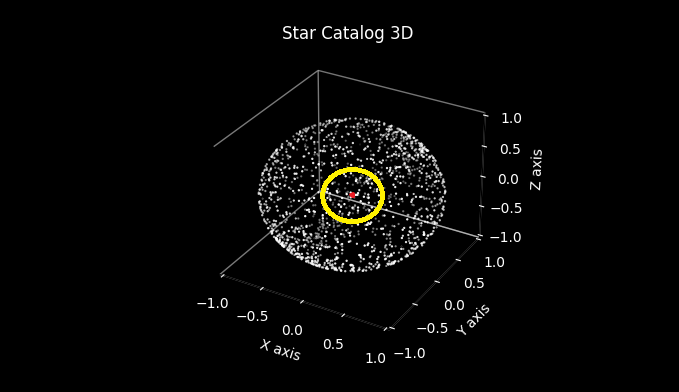
\includegraphics[width=0.8\textwidth]{images/estrelas_endorno.png}
    \caption{Exemplo de Octo Tree, Fonte: \cite{octo_tree}}
    \label{fig:estrelas_endorno}
\end{figure}

Para se localizar de forma eficiente as estrelas ao retor de um circulo no espaço tridimensional, é utilizado a estrutura de dados Octree,
que é uma estrutura de dados que divide o espaço em 8 subespaços, como visto na Figura \ref{fig:octo_tree}. 
Dessa forma, calcula-se apenas areas e ângulos entre estrelas que estão dentro do circulo ao redor da estrela central.

\begin{figure}[H]
    \centering
    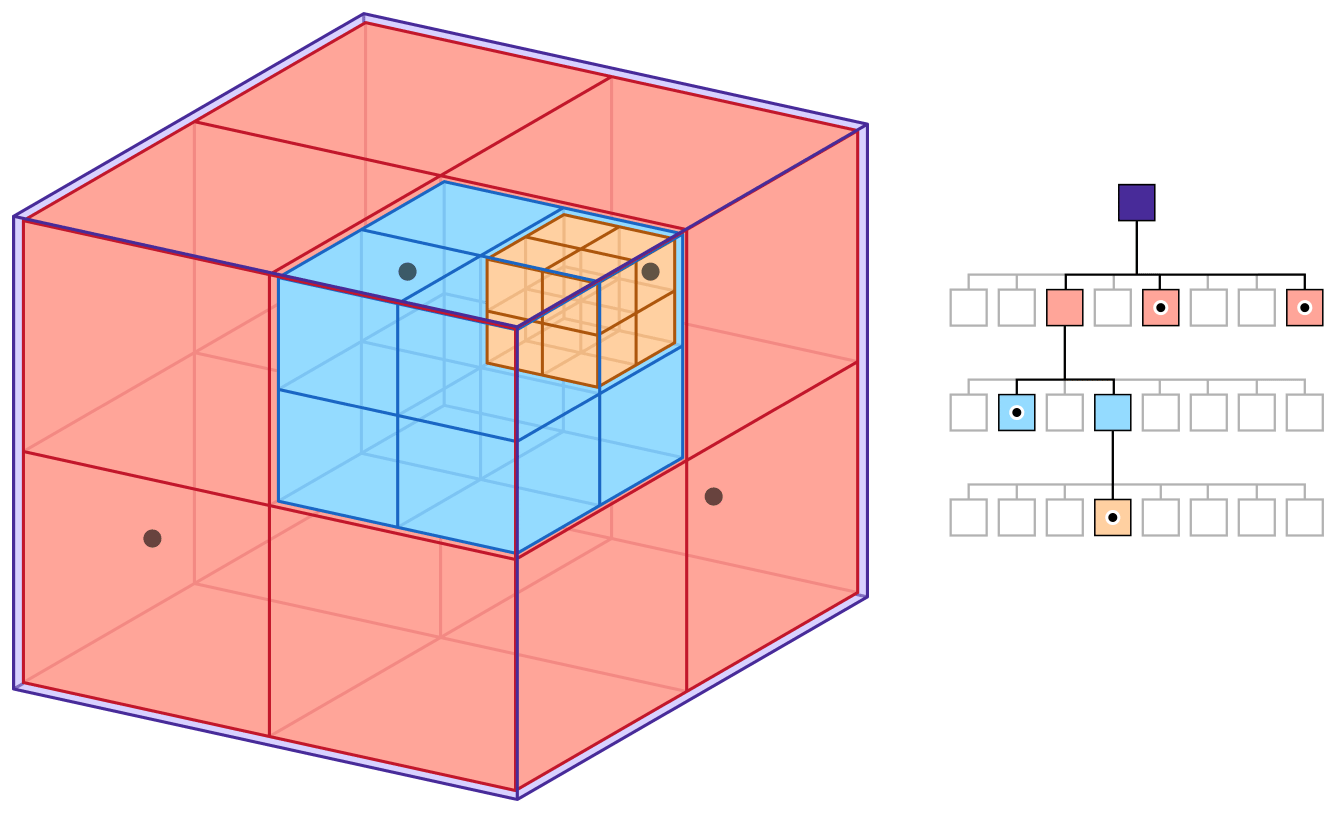
\includegraphics[width=0.8\textwidth]{images/octree.png}
    \caption{Exemplo de Octo Tree, Fonte: \cite{octo_tree}}
    \label{fig:octo_tree}
\end{figure}

\subsubsection{K vector}

O método \textbf{k vector} foi desenvolvido para refinar a faixa de busca em vetores ordenados de dados \cite{Mortari}.
Para que este método seja utilizado é necessário que todos os elementos do banco de dados sejam conhecidos previamente, 
pois o método consiste na criação de um modelo matemático relacionando a informação a ser encontrada, com o index do banco de dados.
Para isso,  a análise é inciada com a ordenação crescente dos dados. 
Apesar de não estritamente necessário, recomenda-se que seja plotado os em um  gráfico cartesiano, como na Figura ~\ref{fig:K_vector}.
Pois a elaboração de uma equação matemática que melhor represente a curva a ser encontrada, é mais fácil de ser feita com a visualização do gráfico.

A Figura ~\ref{fig:K_vector} mostra um exemplo de um gráfico de uma função linear, onde a equação matemática que melhor representa a curva é a equação da reta, 
porém isto não é uma regra, pois a curva pode ser uma função quadrática, cúbica, logarítmica, exponencial, etc.
\begin{figure}[h]
	\centering
	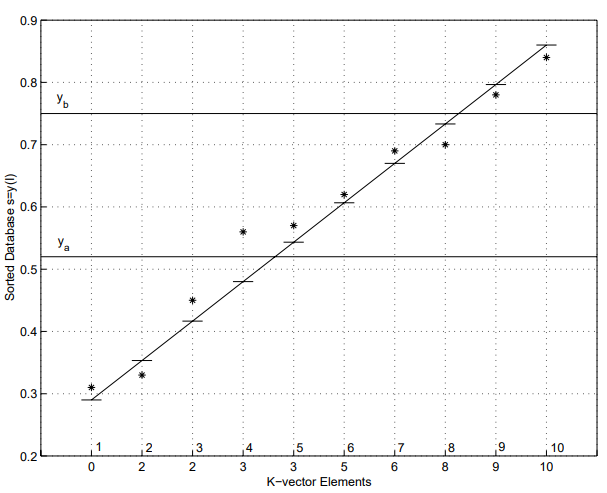
\includegraphics[width=0.5\textwidth]{images/k_vector.png}
	\caption{Exemplo da construção de um K vector. Fonte: ~\cite[]{Mortari}}
	\label{fig:K_vector} 
\end{figure}

No caso apresentado na Figura ~\ref{fig:K_vector}, pode-se utilizar, uma relação linear obtida através do método dos mínimos quadrados pelas equações ~\ref{eq:Beta_linear}, ~\ref{eq:Alpha_linear} e ~\ref{eq:Regressao_linear},

\begin{equation}
	\beta = \frac{\sum_{i=1}^{n} (x_i - \bar{x})(y_i - \bar{y})}{\sum_{i=1}^{n} (x_i - \bar{x})^2},
	\label{eq:Beta_linear}
\end{equation}

\begin{equation}
	\alpha = \bar{y} - \beta * \bar{x},
	\label{eq:Alpha_linear}
\end{equation}

\begin{equation}
	y = \alpha + \beta * x
	\label{eq:Regressao_linear}.
\end{equation}

Para explicar o funcionamento do método, será utilizado o exemplo da Figura ~\ref{fig:covid_1}.
Neste exemplo, objetivo é descobrir o dia em que um numero qualquer de novos casos de covid-19 ocorreram,
dessa forma se utiliza um método de regressão que melhor se encaixa na curva, em teremos como entrda \textbf{x} o numero de casos e como saída \textbf{y} o dia.

\begin{figure}[H]
    \centering
    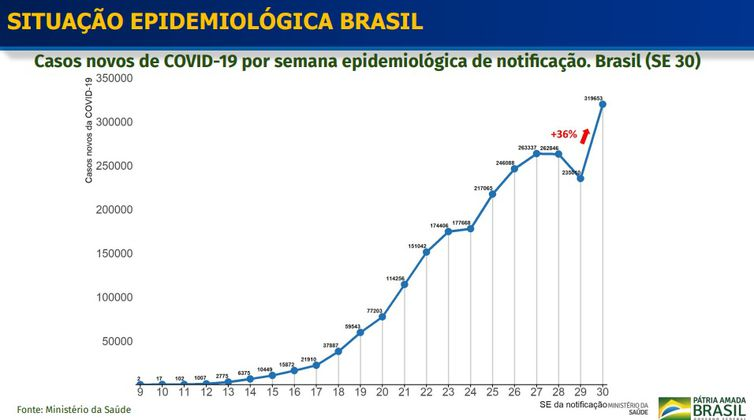
\includegraphics[width=0.5\textwidth]{images/covid_1.jpg}
    \caption{Casos Covid-19. Fonte: ~\cite[]{covid}}
    \label{fig:covid_1}
\end{figure}

Seja a curva vermelha presente na Figura ~\ref{fig:covid_2} a regressão que melhor satisfez aproximação da curva da Figura ~\ref{fig:covid_1}, 
está modelagem matemática apresenta de erros em sua aproximação, como pode se observar no desvio da curva vermelha em relação a curva azul.
Portando além do valor da regressão, é necessário calcular o erro da regressão ~\ref{fig:covid_3}, para que então possa se refinar a pesquisa em apenas uma parte dos set de dados.
Quando então algoritmo de busca binária é utilizado para finalizar a busca.
\begin{figure}[H]
    \centering
    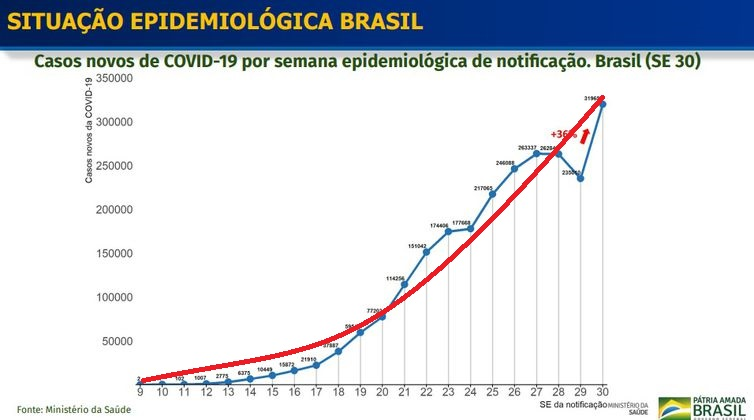
\includegraphics[width=0.5\textwidth]{images/covid_2.jpg}
    \caption{Curva de regressão, Fonte: Autoria Própria}
    \label{fig:covid_2}
\end{figure}

\begin{figure}[H]
    \centering
    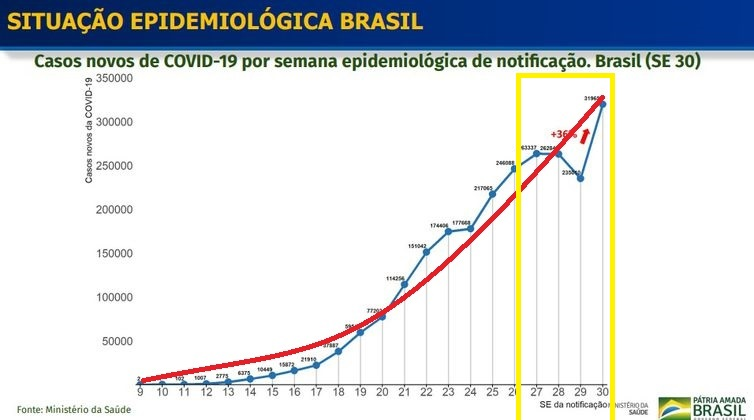
\includegraphics[width=0.5\textwidth]{images/covid_3.jpg}
    \caption{Possíveis dias para um certo numero de casos, Fonte: Autoria Própria}
    \label{fig:covid_3}
\end{figure}

Dessa forma o método consegue diminuir o tempo de pesquisa, ja que um vetor de tamanho \textbf{n}, com todas os valores conhecidos pode ter seu tempo busca reduzido do habitual O(n*log(n)) para O(2*error*log(2*error)), 
diminuí-se o tamanho do vetor de pesquisa a 2 vezes o erro máximo da linearização, dessa forma os algorítimos de busca binária só precisam executar a pesquisa neste vetor selecionado.
Neste trabalho, considero-se que o erro associado a aproximação é, o maior erro entre todos o valor calculado para todos o pontos da curva.

\subsection{Utilizando  o banco de dados}

Após o sistema de analise de imagem, medir os ângulos, areas e momentos triangulares entre as estrelas presentes na imagem, 
o sistema aplica um algótico de seleção de possibilidades, 
onde é selecionado as estrelas que possuem os ângulos e momentos triangulares mais próximos dos valores esperados.

\subsubsection{Pyramid}

Neste trabalho é utilizado o algorítimo de Pyramid, 
o algoritmo funciona da seguinte forma, 
primeiro é selecionado 3 estrelas, \textalpha, \textbeta  e \textgamma, 
com os valores de ângulos juntamente com o erro máximo da medição, é aplicado ao k-vector,
que gera 3 listas diferentes possibilidade.

Com estas listas filtradas é crias-se uma lista com todas as possíveis combinações de 3 estrelas, 
então é analisado o valor de area e momento triangular das estrelas no FOV, filtrado possíveis combinações que não se encaixam nos valores esperados.

Caso a analise resulte em mais de uma combinação possível, é realizado a analise de um segundo triangulo, 
o qual possui pelo menos uma estrela em comum com o primeiro triangulo, 
então o segundo triangulo é analisado da mesma forma que o primeiro.
Então os resultados dos dois triângulos são comparados, para selecionar apenas as possibilidades que estão presentes nos dois resultados.

Pode se visual o processo nas figuras ~\ref{fig:pyramid_1} e ~\ref{fig:pyramid_2} e ~\ref{fig:pyramid_3}.
\begin{figure}[H]
    \centering
    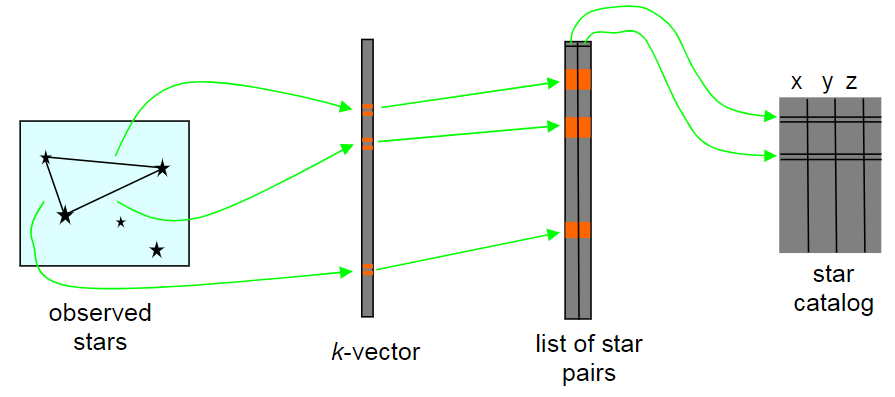
\includegraphics[width=1\textwidth]{images/Pyramid_01.png}
    \caption{Pyramid, Fonte: ~\cite[]{Fialho}}
    \label{fig:pyramid_01}
\end{figure}


\begin{figure}[H]
    \centering
    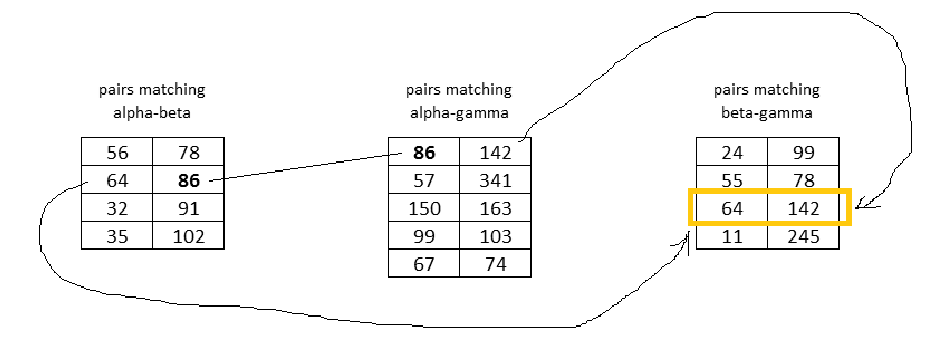
\includegraphics[width=1\textwidth]{images/Pyramid_02.png}
    \caption{Exemplo de Pyramid, Fonte: ~\cite[]{Fialho}}
    \label{fig:pyramid_02}
\end{figure}

\begin{figure}[H]
    \centering
    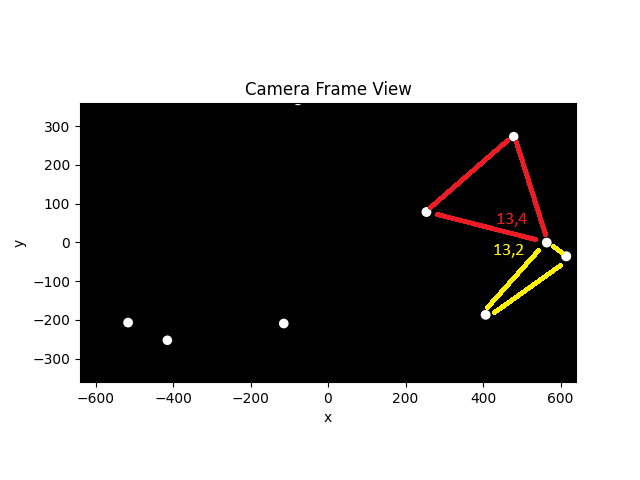
\includegraphics[width=1\textwidth]{images/Pyramid_03.png}
    \caption{Exemplo de Pyramid, Fonte: Autoria Própria}
    \label{fig:pyramid_03}
\end{figure}

No exemplo da Figura ~\ref{fig:pyramid_03}, a estrela que faz parte dos dois triângulos pode ser 13, 2 segundo a analise do triangulo amarelo, 
segundo a outra analise de pode-ser 13, 4 portando está estrela deve ser a 13.

%\chapter{Simulação}
\section{Objetivo}

O objetivo da simulação é poder realizar teste em ambiente controlado, de forma a se averiguar a precisão, acurácia e velocidade de processamento da posição por parte do Star Tracker. Para isto, a simulação deve implementar modelos matemáticos que representem o sistema real o mais fielmente possível.

\section{Recursos e características}

\textbf{GUI (Graphical User Interface):} A simulação é inteiramente controlada através de uma GUI criada para facilitar o controle e a execução dos testes, também é utilizada para facilitar a visualização e a correção de possíveis erros e bugs no software e no desenvolvimento do trabalho em geral. A implementação dos módulos de funcionamento do software segue conceitos dos TDD (Test driven  development), juntamente da arquitetura de software MVC (model view controller), para organizar o funcionamento da interface em si.

\textbf{Gerador de campo de visão:} Esta é a função principal do software de simulação, que é gerar uma janela com o campo de visão que teoricamente seria visto pela câmera, a imagem gerada é monocromática com as estrelas projetadas sobre a superfície plana do monitor, neste trabalho as estrelas simuladas são apenas círculos brancos em um fundo preto, porém são estrelas retiradas de uma base de dados reais.

\textbf{Load de arquivos:} Para facilitar a mudança de parâmetros durante os testes e simulações , o software carrega todas as informações inerentes a configuração e execução dos testes, através de caixas de diálogo que pedem a seleção dos arquivos de simulação. Para uma maior modularidade, cada informação está dividida em arquivos diferentes, com arquivos separados para configuração de câmera, base de dados de estrelas e sequência de movimentos a ser realizada.

\textbf{Elementos auxiliares de visualização:} Além das funcionalidades básicas, o software implementa  recursos de configuração  de aspectos visuais. Apesar de não serem estritamente necessários são de extrema importância  para análises menos rigorosas das informações, como por exemplo, o plot 3D, a projeção cartográfica em 2D. Com opções de visualização da posição das câmeras e demais auxílios.

\textbf{Controles manuais e automáticos:} O software possui controles manuais de rotação, que permitem a rotação da simulação em todos os 3 eixos de liberdade, através de configurações na GUI, além disto o usuário pode preparar uma sequência de movimentos e suas respectivas durações previamente.

\textbf{Salvar frames:} O usuário pode salvar frames de imagem em arquivos png para facilitar a utilização posterior da posição.

\section{Projeção em perspectiva}

A projeção descreve matemática como representar um ponto com 3 graus de liberdade, no espaço bidimensional do monitor e do frame da câmera. Essa transformação pode ser realizada através de matrizes, que levam em consideração elementos como o ângulo focal da lente, a resolução e proporção da imagem.

\subsection{Square Frustum}

Frustum retangular é um espaço que contém a linha de visão de  um visualizador como se este possuísse um ângulo de visão retangular, que é caso de câmeras com CCD retangulares, para melhor entender este conceito recomenda-se a observação da Figura \ref{fig:frustum}.

\begin{figure}[h]
    \centering
    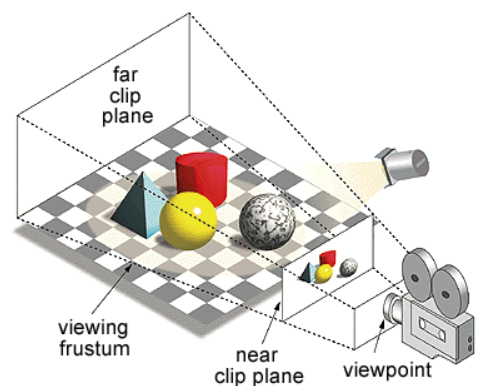
\includegraphics[width=0.5\textwidth]{images/frustum.png}
    \caption{Visualização Frustum rectangular, Fonte: ~\cite[]{the_free_dictionary}}
    \label{fig:frustum}
\end{figure}

A existência de um plano ao fundo na cena (far clip), se deve ao equacionamento que leva os pontos presentes na cena 3D para o frame 2D da câmara, além de reduzir o custo de processamento requerido pelo programa para gerar a cena sendo parte importante do equacionamento do frame da câmera.

Considerando que o ângulo de visão da câmera esteja apontada para o positivo do eixo x como é mostrado na figura \ref{fig:posicao_inicial_camera}.

\begin{figure}[h]
    \centering
    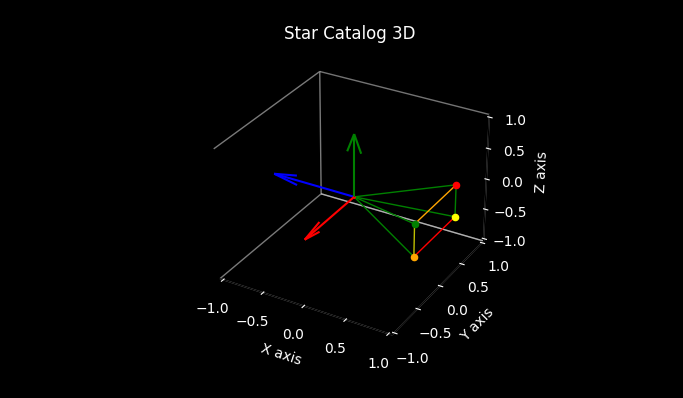
\includegraphics[width=0.5\textwidth]{images/posicao_inicial_camera.png}
    \caption{Visualização da câmera na posição inicial}
    \label{fig:posicao_inicial_camera}
\end{figure}

As setas coloridas presentes na imagem são as coordenadas do frame da câmera, que seguem um esquema de cores usual para esse tipo de aplicação, na figura 17 é demonstrado as relações X,Y e Z com as cores:



\begin{figure}[h]
    \centering
    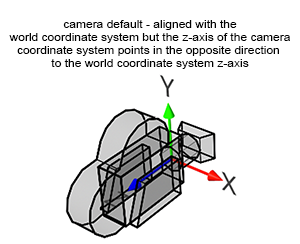
\includegraphics[width=0.5\textwidth]{images/coordenadas.png}
    \caption{Coordenadas do frame da camera. Fonte: ~\cite[]{the_free_dictionary}}
    \label{fig:coordenadas}
\end{figure}


Com isso se desenvolveu a seguinte equação matricial da câmera, seguindo os passos mostrados por Brendan Galea em seu video ~\cite[]{Galea}:

\begin{equation}
    \begin{bmatrix}
        x' \\
        y' \\
        z' \\
        w
    \end{bmatrix}
    =
    \begin{bmatrix}
        \frac{f+n}{f-n} & 0                                 & 0                               & \frac{-2fn}{f-n} \\
        0               & \frac{h}{w*tan(\frac{\theta}{2})} & 0                               & 0                \\
        0               & 0                                 & \frac{1}{tan(\frac{\theta}{2})} & 0                \\
        1               & 0                                 & 0                               & 0
    \end{bmatrix}
    \begin{bmatrix}
        x \\
        y \\
        z \\
        1
    \end{bmatrix}
\end{equation}

Em que, \textbf{f} é a distância do far plane ao ponto (0,0,0), que neste caso é sempre unitário já que a estrelas estão presentes em um círculo unitário, $\Theta$ é o ângulo de abertura  da câmera, \textbf{w} é a quantidade de pixels na horizontal camera, \textbf{h} é quatidade e pixel na vertical da câmera por fim \textbf{n} é a distância do near plane, que neste caso é o coseno de $\frac{\Theta}{2}$.

Nota-se que a matriz de transformação da câmera é uma matriz 4X4 isso ocorre pois as equações de transformação são realizadas através de coordenadas homogêneas e não coordenadas cartesianas tradicionais.

Além da matriz, existe uma equação de clipping que determina se uma estrela deve ou não aparecer no frame, devido a simplicidade da simulação aqui implementada essa equação se tornou apenas um cheque se a estrela se encontrava na metade da esfera celeste em que x é positivo.

O resultado dessa simulação pode ser visto na Figura \ref{fig:resultado_simulacao}.

\begin{figure}[h]
    \centering
    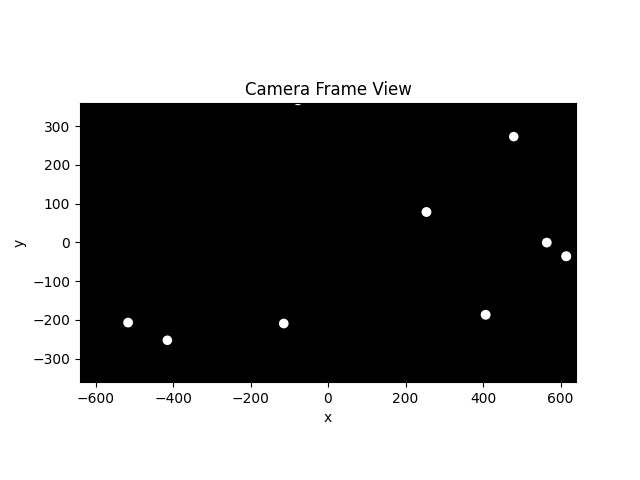
\includegraphics[width=\textwidth]{images/resultado_simulacao.png}
    \caption{Camera frame at position,declination 0º, arcensão 0º, roll 0º}
    \label{fig:resultado_simulacao}
\end{figure}

%\include{rotacao.tex}

%\section{Desenvolvimento de software}

\subsection{Test Driven Development(TDD)}

O  Desenvolvimento Orientado a Testes,  consiste em desenvolver testes separados para cada parte de um software como é o caso das funções, os testes devem garantir que o código funcione e cumpra a tarefa desejada.

Para aplicá-lo, primeiro cria-se o teste ,dessa forma garante-se que o que durante o desenvolvimento do código o resultado inicialmente esperado seja obtido, dessa forma o teste falha na primeira vez que é executado, já que este está testando o recurso que ainda não existe, em seguida é desenvolvido o recurso de forma a fazer o teste passar, então repete-se este ciclo função por função. 

Caso seja localizado um bug no software, primeiramente o desenvolvedor deve implementar um teste que consiga replicar o erro em específico, só então a realizar a correção, dessa forma se garante a correta implementação da solução, assim como o novo software deve manter-se passando nos testes anteriores. Algumas das vantagem de tal método são:
\begin{itemize}
    \item Facilidade em focar em problemas específicos de desenvolvimento
    \item Códigos são fáceis de refatorar
    \item Facilidade em corrigir bugs, mesmo durante o desenvolvimento
    \item Capacidade em garantir do que está funcionando e como está funcionando
    \item Dividir de forma mais clara cada parte do código 
    \item Descobrir falhas de forma prematura durante o processo de desenvolvimento
    \item Maior organização de código
\end{itemize}

Como este projeto é desenvolvido em python, é utilizado o framework pytest, para implementação dos testes, ressalta-se também que apenas os módulos do software responsáveis por realizar a matemática aqui aplicada e desenvolvida, que foram testados por tal metodologia, com a parte do software relacionada a interfaces gráficas não sendo desenvolvidas dessa forma, isto ocorre pois apesar de ser perfeitamente possível de se utilizar TDD, a criação de testes para tais componentes de software costuma ser lenta e difícil, optando-se então por apenas realizar checks visuais neste caso.

\subsection{Model View Controller (MVC)}
MVC é um arquitetura de software desenvolvida para otimizar o processo de desenvolvimento de interfaces gráficas, com foco em diminuir o tempo de manutenção do código, facilitando o debug de elementos visuais do sistema, também facilita a interação de múltiplos desenvolvedores e proporciona uma maior clareza de código exigindo um baixo nível de acoplamento entre as partes. 

Para isso o MVC se divide em 3 componentes principais, o model, o controller e o view, as regras de negócio estão contidas no model assim como as informações  necessárias para execução do programa o controller realizar a interface entre o model e view, que contém as especificações de como os usuários interagem com o sistema.

O view decide como apresentar as informações e como os inputs de informações são feitos, por exemplo o usuário ao clicar em um botão que tem sua aparência e posição especificados pelo view, gera um evento que é tratado pelo controlador que se preciso for irá formatar os dados gerados pela interface então transfere o dado para o model, que executa a aplicação em si, como por exemplo realizando equações matemáticas, carregando arquivos e demais lógicas de negócio.

O model também é responsável por armazenar as informações sobre o estado de execução do sistema.

No simulador estrelar aqui desenvolvido utiliza-se 3 views separados, para gerenciar diferentes janelas de usuário, com um único modelo que é responsável por armazenar a lógica de negócios, que consiste na execução dos códigos de simulação.


% --- Finaliza a parte no bookmark do PDF, para que se inicie o bookmark na raiz ---
\bookmarksetup{startatroot}%
% ---

% --- Conclus\~{a}o ---
%\chapter*[Conclusão]{Conclusão}
\label{cap:Conclusao_init}
\addcontentsline{toc}{chapter}{Conclusão}


Ao longo do desenvolvimento deste trabalho, vários pontos de melhorias fora notados, 
assim como pontos de desenvolvimento futuros, o que envolve melhorias e adições ao Star Tracker em si, 
mas também envolvem a integração do sistema aqui desenvolvido com outros outros componentes do sistema de orientação espacial do cubesat,
é listado uma series de pontos a serem trabalhados.

Além disto alguns erros de arquitetura do sistema cometidos pelo autor, não permitiram a analise com grandes conjuntos de dados, 
com diferentes frames, porém o sistema se mostra promissor.

\section*{Correções e testes adicionais}
\begin{itemize}
	\item \textbf{Melhorias na implementação do algoritmo de correção de distorções}: Apesar da correção da distorção de pixel parecer aceitável, 
	pelos resultados apresentados na seção anterior, a incidência de erros na resposta final de detecção de estrelas, indica que esta etapas pode conter erros, 
	uma das possíveis soluções, é a utilização da biblioteca open CV para realizar esta etapa, pois esta já possuir algorítimos para resolução de distorções, 
	porém houve uma escolha de não ha utilizar pois está implementa uma serie de recursos matemáticos ainda não completamente entendidos pelo autor. 
	\item \textbf{Utilização do triângulos esféricos}: Neste trabalho utiliza-se triângulos planares, porém a utilização de triângulos esféricos aumenta a precisão do sistema, 
	como é explicado por Cole ~\cite{Cole_2}
	\item \textbf{Refatoração da estrutura de testes}: A atual estrutura de testes é pensada para ser de fácil compressão, 
	e permitir o teste de diferentes senários pelo usuário, porém o deste em milhares de entradas para se fazer analises estatísticas melhores não é possível de forma fácil, 
	isto não se deve a limitações de algorítimo, pois o algoritmo ao al do tipo, mas sim um erro estrutural de organização de testes.
	Portanto a refatoração destes códigos se faz necessária para um melhor desenvolvimento de etapas futuras. 
\end{itemize}

\section*{Perspectivas Futuras}

\begin{itemize}
	\item \textbf{Desenvolvimento de um simulador para teste de hardware}: Esta etapa já foi descrita na seção ~\ref{cap:simulador}
	\item \textbf{Construção física de um sistema de câmera}: A construção de um sistema físico, para deste mais fieis a realidade também se faz necessária, 
	nota-se que ao longo deste trabalho todos os códigos foram testado em raspberry pi 4, o que facilita muito no desenvolvimento ode futuras etapas. 
	\item \textbf{Integração com filtro dde Kalman}: Com o protótipo físico em mão pode se iniciar a integração com outros sistema de metição para se refinar a precisão.
\end{itemize}

% ---- ELEMENTOS P\'{O}S-TEXTUAIS ----
\postextual

% ---- Refer\^{e}ncias bibliogr\'{a}ficas ----
\bibliography{tese}

% ---- Ap\^{e}ndices ----

% ---
% Inicia os ap\^{e}ndices
% ---
\begin{apendicesenv}

%\include{apendice}

\end{apendicesenv}
% ---

% ---- Anexos ----

% ---
% Inicia os anexos - opcional
% ---
%\begin{anexosenv}
%
%% Imprime uma p\'{a}gina indicando o in\'{\i}cio dos anexos
%\partanexos
%
%% ---
%\chapter{Morbi ultrices rutrum lorem.}
%% ---
%\lipsum[30]
%
%\end{anexosenv}
%
%% ---- INDICE REMISSIVO ----
%
%\printindex

\end{document} 